\documentclass[12pt,a4paper]{article}
\usepackage[margin=26mm,headheight=16pt]{geometry}
\usepackage[T1]{fontenc}
\usepackage[utf8]{inputenc}
\usepackage{lmodern,microtype,parskip,setspace,ragged2e}
\usepackage{xcolor,graphicx,booktabs,tabularx,array,enumitem,titlesec,fancyhdr}
\usepackage[most]{tcolorbox}
\usepackage{tikz}
\usetikzlibrary{arrows.meta,positioning,fit}
\usepackage[colorlinks=true,linkcolor=teal!60!black,urlcolor=teal!60!black]{hyperref}
\definecolor{teal}{HTML}{187C80}
\definecolor{pale}{HTML}{EEF6F5}
\definecolor{ink}{HTML}{203342}
\setstretch{1.20}
\setlength{\parindent}{0pt}
\setlength{\parskip}{0.8em}
\setlist[itemize]{leftmargin=1.4em,itemsep=0.45em,topsep=0.4em,parsep=0.15em}
\setlist[enumerate]{leftmargin=1.5em,itemsep=0.5em,topsep=0.4em,parsep=0.15em}
\titlespacing*{\section}{0pt}{1.5em}{0.7em}
\titlespacing*{\subsection}{0pt}{1.2em}{0.5em}
\widowpenalty=10000
\clubpenalty=10000
\setlength{\emergencystretch}{2em}
\pagestyle{fancy}
\fancyhf{}
\lhead{\small Day 1 | ML architecture}
\rhead{\small Bank customer-churn example}
\cfoot{\thepage}
\renewcommand{\headrulewidth}{0.3pt}
\tcbset{breakable,arc=1.5mm,boxrule=0.6pt,left=3mm,right=3mm,top=2.5mm,bottom=2.5mm,before skip=12pt,after skip=12pt,fonttitle=\bfseries,before upper={\setlength{\parskip}{0.6em}\RaggedRight}}
\newtcolorbox{keybox}[1]{colback=pale,colframe=teal,title={#1}}
\newtcolorbox{examplebox}[1]{breakable=false,colback=orange!5,colframe=orange!55!black,title={At our bank: #1}}
\newtcolorbox{handoffbox}[1]{colback=blue!3,colframe=blue!40!black,title={#1}}
\newcommand{\source}[1]{\par\textcolor{teal!70!black}{\textit{Reading anchor: #1}}\par}
\begin{document}
\RaggedRight
\title{One Bank, One Story\\[0.4em]\large A detailed Day 1 handoff for the presentation team}
\author{Ricardo, Tomás, Simon, Luca, and Matheus}
\date{Classical ML architecture --- 20 October 2026}
\begin{center}
{\LARGE One Bank, One Story\par}
{\large A detailed Day 1 handoff\par}
Ricardo, Tomás, Simon, Luca, and Matheus\\
Classical ML architecture --- 20 October 2026
\end{center}

\begin{keybox}{What we want the audience to follow}
A bank learns to estimate customer churn. We put the model into use, notice a problem, diagnose its architectural causes, repair the change process, and review the system's quality and safeguards.

Each speaker advances that same story. We organize by the questions the bank must answer, bringing the readings into the relevant step.
\end{keybox}

\textbf{How to use this handoff.} Everyone should read Sections 1--3. Then read your own step and the steps immediately before and after it. Each step identifies what to explain, what happens to our example, what to show, and a suggested handoff sentence.

The timings are a proposed 60-minute speaking plan. Quality-checklist and tool-showcase ownership remain \textbf{TBD}. Security and privacy retain the existing joint assignment to \textbf{Simon and Matheus}.


\section{Agree on the example before making slides}
\subsection{The bank's goal}
Our bank wants to identify customers who may leave soon enough to make a helpful retention decision. \textbf{Churn} means ending the customer's relationship with the bank, rather than merely logging in less often.

The customer-churn case in Bass et al., Chapter 14, is our foundation. It includes source data, prepared features, model training, stored scores, campaign use, monitoring, and banking-specific concerns.

The model estimates risk. A separate campaign process decides whether and how to act. For example, a high score should not override a customer's contact preferences.

\subsection{Our simplified teaching contract}
Use these choices consistently across sections and slides:
\begin{itemize}
\item \textbf{One main task:} estimate which existing customers will leave during the next 30 days. The exact outcome definition and window are choices for our teaching version; Bass describes about a month's lead time.
\item \textbf{One main serving mode:} a monthly batch scores many customers and saves the results. Bass describes batch predictions at intervals such as fortnightly or monthly.
\item \textbf{One model output:} an estimated churn-risk score. A score is neither a decision to send an offer nor certainty about the customer's future.
\item \textbf{One downstream action path:} campaign policy checks preferences, eligibility, contact limits, and the budget before staff or a campaign system acts.
\item \textbf{One feedback path:} after the outcome window closes, observed churn labels are linked to the original scores to evaluate quality.
\end{itemize}

These choices make the example concrete. They are not a claim that Bass's bank used every detail of our proposed design.

\subsection{Meet Ana: the record everyone reuses}
Ana is fictional. Her teaching identifier is \texttt{C042}; all values below are invented.

\begin{examplebox}{Ana on the scoring date}
The bank has historical account, transaction, app-use, and customer-interaction records. One prepared input says that Ana's app logins fell from seven in the previous week to one in the latest week.

The model produces a risk score of \textbf{0.70}. The campaign system then checks whether contact is appropriate. Ana's actual churn outcome is still \textbf{unknown} on this date.
\end{examplebox}

A \textbf{feature} is a prepared model input, such as the seven-day login count. A \textbf{label} is the observed outcome used for learning or evaluation. A \textbf{model version} identifies the particular learned rule used to produce a score.

Ana's lower app activity is a useful illustration of a feature. It is not proof that she wants to leave. An explanation of which inputs affected her score is also not a causal explanation of her behavior.

\section{The shared system and the recurring incident}
\subsection{Follow the same data-to-action path}
\begin{enumerate}
\item \textbf{Source records.} Core banking, CRM, payment, and app systems supply data. Someone owns each source and its changes.
\item \textbf{Prepared features.} The pipeline validates records, joins them correctly, and computes inputs such as recent login counts. Definitions and time windows must be consistent.
\item \textbf{Training and evaluation.} Historical features and known labels support candidate models. The team compares candidates and records the code, data, and configuration behind them.
\item \textbf{Approved model and batch scoring.} A selected model is packaged and registered. The production job combines that version with current prepared features to generate a score batch.
\item \textbf{Campaign decision.} The campaign process uses scores alongside business rules. It records what action, if any, was taken.
\item \textbf{Monitoring and outcomes.} Operational checks run immediately. Model-quality evaluation follows when labels are ready. Evidence can prompt investigation, repair, rollback, or a new candidate.
\end{enumerate}

\begin{figure}[htbp]
\centering
\resizebox{0.98\textwidth}{!}{%
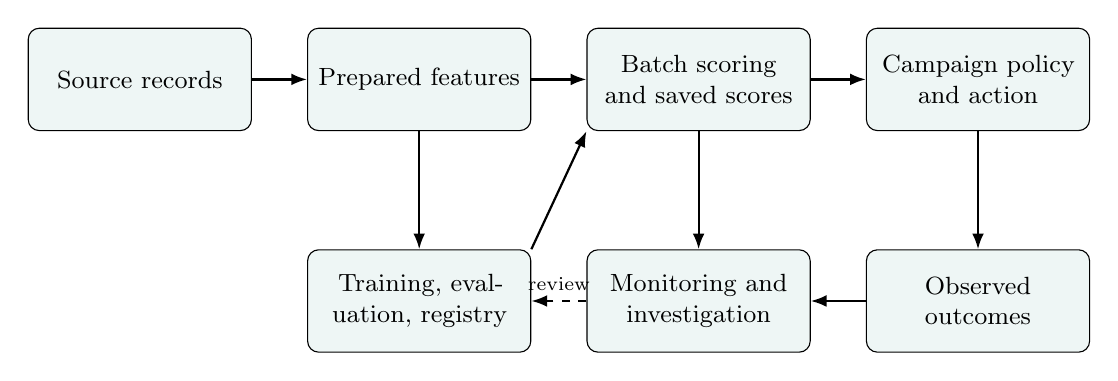
\begin{tikzpicture}[node distance=9mm and 7mm,box/.style={draw,rounded corners,align=center,text width=26mm,minimum height=13mm,fill=pale,font=\small},arr/.style={-{Latex[length=2mm]},thick}]
\node[box] (sources) {Source records};
\node[box,right=of sources] (features) {Prepared features};
\node[box,right=of features] (scores) {Batch scoring and saved scores};
\node[box,right=of scores] (campaign) {Campaign policy and action};
\node[box,below=15mm of features] (training) {Training, evaluation, registry};
\node[box,below=15mm of scores] (monitor) {Monitoring and investigation};
\node[box,below=15mm of campaign] (outcome) {Observed outcomes};
\draw[arr] (sources)--(features); \draw[arr] (features)--(scores); \draw[arr] (scores)--(campaign);
\draw[arr] (features)--(training); \draw[arr] (training.north east)--(scores.south west);
\draw[arr] (scores)--(monitor); \draw[arr] (campaign)--(outcome); \draw[arr] (outcome)--(monitor);
\draw[arr,dashed] (monitor)--node[above,font=\scriptsize]{review}(training);
\end{tikzpicture}}
\caption{The reusable teaching diagram, adapted from the bank case's activities. The dashed arrow means review can request a change; an alarm does not automatically approve a new model.}
\end{figure}

\subsection{Introduce one incident and resolve it together}
After a successful deployment, a CRM migration makes the engagement feature missing for a subset of customers. The model has not changed. Some scores may now be unreliable.

This is our fictional recurring incident. Simon detects it; Luca explains the dependency and design weaknesses; Matheus shows the controlled repair and release path. Simon and Matheus then ask how that same path would resist a malicious source change.

A separate concept-drift illustration can show how customer behavior changes over time. Do not call the CRM fault concept drift unless the relationship between valid inputs and churn has actually changed.

\subsection{What stays identical across everyone's slides}
Use the same customer identifier, input definition, model-version label, pipeline boxes, and direction of arrows. Highlight the box your section is discussing rather than replacing the diagram with an unrelated architecture.

The example remains bank churn. Real-time fraud detection is a brief comparison when Tomás explains a different serving requirement. Edge deployment is assessed as an alternative location, rather than added as another component the bank must build.

\source{Bass, \S14.1--14.2; Kalinowski, \S13.2--13.4. Diagram and incident are team teaching syntheses.}

\section{The proposed speaking sequence}
\begin{tabularx}{\textwidth}{@{}p{0.19\textwidth}X@{}}
\toprule
\textbf{Time} & \textbf{Owner and question}\\
\midrule
0--8 min & Ricardo: what makes this a system problem rather than only a model problem?\\
8--17 min & Tomás: how do approved predictions reach the campaign?\\
17--26 min & Simon: how do we notice and respond when the deployed system becomes unreliable?\\
26--35 min & Luca: which dependencies and design choices make change difficult or manageable?\\
35--44 min & Matheus: how do we make the change process repeatable and traceable?\\
44--51 min & Simon + Matheus: who can interfere with the pipeline, and what customer information should it expose?\\
51--56 min & TBD: does the design meet our quality concerns, and what evidence supports that?\\
56--60 min & TBD / all: which practical tools support the design, and what did the example teach us?\\
\bottomrule
\end{tabularx}

The shared diagram provides the architectural foundations throughout. Ricardo introduces its responsibilities; Luca develops the separation and change trade-offs. If the group wants a standalone foundations segment, agree on its owner and reduce time elsewhere.

\section{Step 1 --- Ricardo: establish the model-to-system problem}
\textbf{Story beat:} the bank has a useful predictive idea, but it needs more than a trained model to act on it.

\subsection{What to explain, in order}
\begin{enumerate}
\item Introduce churn, the retention goal, and Ana's record. Define data, feature, model, and label before using the full pipeline diagram.
\item Explain the \textbf{software lifecycle}: developers change code, integrate it, test it, and release it. A contact-frequency rule or a CRM connector can change even if the learned model remains the same.
\item Explain the \textbf{model/data lifecycle}: collect examples, prepare features, train, evaluate, and eventually update the learned rule. Outcome labels arrive on a different schedule from code changes.
\item Connect the two lifecycles. A model depends on data meanings and preparation code; a release must keep these compatible. Predictive uncertainty does not mean every execution of a fixed model is random.
\end{enumerate}

\textbf{Use the example.} Ana can be scored today, but her 30-day label is not yet available. A software test can check that the scoring job runs. It cannot tell us today whether that particular prediction will later be correct.

\textbf{Show the audience.} Use two short lanes, ``software changes'' and ``data/model changes,'' converging on an approved production version. Then place Ana's record on the shared diagram. Keep the lifecycle recap brief because earlier course presentations already covered it.

\source{Kalinowski, \S13.2; Bass, \S14.1--14.1.4; Nazir, introduction and lifecycle-related decisions. The two-lane illustration is our synthesis.}

\begin{handoffbox}{Handoff to Tomás}
``We now know what the bank must learn and what the surrounding software must do. How does an approved model actually deliver scores to the campaign team?''
\end{handoffbox}

\section{Step 2 --- Tomás: put the model into use}
\textbf{Story beat:} the bank moves from a trained artifact to a reliable flow of usable predictions.

\subsection{What to explain, in order}
\begin{enumerate}
\item Walk through the normal batch path: validate current data, compute features, load an approved model, score customers, and save results for the campaign. Tie the completion deadline to campaign needs.
\item Distinguish \textbf{prediction modes}. Batch precomputes many scores. A synchronous caller waits for a response. In an asynchronous design, events and predictions travel through messaging so components do not need the same immediate call-and-response sequence.
\item Distinguish \textbf{deployment location}. Embedded or edge inference runs near the device. It is a different design dimension from batch versus online. Explain why our centrally governed churn workflow uses the batch path.
\item Explain packaging and release separately. Packaging includes the model, required dependencies, input expectations, and feature compatibility. A release strategy controls how a new version is introduced.
\end{enumerate}

\subsection{Use the same example for release strategies}
\textbf{Shadow:} a candidate scores the same customer batch as the current model, but its outputs do not trigger offers. Compare execution, score differences, and eventual quality.

\textbf{Canary:} a limited, approved customer cohort uses the new version while most remain on the old one. This limits exposure. Passing early operational checks does not replace waiting for meaningful churn outcomes.

\textbf{A/B test:} allocate comparable groups to defined alternatives to evaluate a stated outcome. Be explicit whether the experiment changes the model or the retention treatment; otherwise their effects become difficult to interpret.

These are proposed applications to our bank. Kalinowski supplies the prediction architectures; Breck et al. supplies supplementary support for gradual introduction and rollback.

\textbf{Show the audience.} Highlight scoring and the score table on the shared diagram. Add a small current-model/candidate branch with a clear switch indicating whether a score may trigger a campaign. Ana should not receive duplicate offers because two models ran.

\source{Kalinowski, \S13.3--13.4 and supporting Ch. 12; Bass, \S14.1.4; Breck et al., infrastructure tests 6--7.}

\begin{handoffbox}{Handoff to Simon}
``The first scoring run worked, and the campaign can use its results. What evidence tells us that the system remains reliable after source data and customer behavior start changing?''
\end{handoffbox}

\section{Step 3 --- Simon: notice the incident and choose a response}
\textbf{Story beat:} the deployed model stays unchanged, but the CRM migration makes part of its input unreliable.

\subsection{What to explain, in order}
\begin{enumerate}
\item Begin with the missing engagement feature, not with a list of drift definitions. Show the affected cohort and the source-change timing.
\item Separate four possible causes: a data-quality fault, different training/serving preparation, changed input distributions, and a changed input-to-churn relationship. Explain why one statistical alarm does not identify all four.
\item Separate immediate checks from delayed model evaluation. Freshness, missingness, batch completion, and score distributions can be checked now. Precision, recall, and calibration for the full churn window need mature labels.
\item Explain the response: investigate, pause questionable actions or use an appropriate fallback, repair or roll back where justified, and evaluate a new candidate only when evidence supports it.
\end{enumerate}

\textbf{Use the example.} Ana's engagement feature is now missing because the CRM import changed. The bank should not confidently reinterpret that missing value as customer disengagement. Retraining on the defective records could preserve the defect in the next model.

\textbf{Show the audience.} Put a warning on the source-to-feature arrow. Show a short incident timeline: migration, missingness alarm, affected-cohort investigation, temporary response, validated repair. Add a second timeline showing why churn labels arrive later.

\textbf{Your response boundary.} Explain what evidence requests repair, rollback, or retraining. Leave the detailed automated checks, artifact recording, and promotion mechanism to Matheus. Leave the structural dependency decisions to Luca.

\source{Bass, \S14.1.1, \S14.1.5 and Ch. 11; Kalinowski, \S13.2; Breck et al., Section V.}

\begin{handoffbox}{Handoff to Luca}
``We found the immediate data fault. Why could a change in another team's CRM system reach our predictions so easily, and which design decisions would make the next change easier to manage?''
\end{handoffbox}

\section{Step 4 --- Luca: explain dependencies and design for change}
\textbf{Story beat:} the incident exposes hidden dependencies, rather than proving that the model algorithm was badly chosen.

\subsection{Develop three concrete decisions}
\begin{enumerate}
\item \textbf{Make the input contract explicit.} State the feature's meaning, time window, allowed missing values, owner, and compatibility expectations. Link a source change to its downstream consumers. This contract is our proposed response to the bank's dependency problem.
\item \textbf{Separate responsibilities.} Keep loading, feature preparation, model execution, and campaign rules as identifiable parts. A CRM repair belongs to data preparation; a contact rule belongs to campaign policy. Separate responsibilities do not automatically require separate network services.
\item \textbf{Track compatible versions.} Record which data definition, feature code, model, and configuration belong together. A model version alone cannot explain Ana's score if its inputs silently changed meaning.
\end{enumerate}

\subsection{Make patterns concrete without a code lecture}
Kalinowski's \textbf{Pipeline} pattern breaks processing into smaller steps. Use it to show where validation belongs before scoring.

The \textbf{Strategy} pattern provides an interface for replacing one algorithm or preparation strategy. A controlled change to feature selection can use that interface; it still requires evaluation.

The \textbf{Observer} pattern lets a monitoring component notify another component of a change. Notification requests investigation; it does not grant permission to promote a new model.

The single-responsibility principle and dependency injection support clearer responsibilities and replaceable dependencies. Explain one design boundary well rather than listing every SOLID principle and pattern.

\textbf{Show the audience.} Contrast an implicit ``CRM table feeds model'' arrow with an explicit validation-and-feature boundary. Annotate which part changes during the repair and which artifact links must be recorded.

\textbf{Discuss a trade-off.} More services can improve independent change but add network, deployment, and recovery work. Nazir reports context-dependent decisions and evidence gaps; it does not establish microservices as the best answer for every ML system.

\source{Nazir, Sections 5--6, especially architecture and data/evolution/QA decisions; Kalinowski, \S14.2--14.4; Bass, \S14.1.1.}

\begin{handoffbox}{Handoff to Matheus}
``We have clearer responsibilities and know which versions must remain compatible. How do we make that design a repeatable process instead of relying on someone to remember every check?''
\end{handoffbox}

\section{Step 5 --- Matheus: make change repeatable and traceable}
\textbf{Story beat:} the team repairs the CRM path through a controlled process and can explain exactly what changed.

\subsection{Walk one change through the pipeline}
\begin{enumerate}
\item \textbf{Record the change.} The repair has reviewed code, a data/feature definition, and an identified configuration. These identify what is being released.
\item \textbf{Check compatibility.} Test that the corrected source records produce valid features and the approved model accepts them. Check the complete path to stored scores, not only a standalone model function.
\item \textbf{Train only if needed.} The CRM repair may require recomputing scores with the current model rather than retraining. If a new candidate is justified, evaluate it on suitable data and important customer groups.
\item \textbf{Register and promote.} Store the model artifact and links to its training run, code, data, dependencies, and evaluation. Apply a release gate, use Tomás's chosen rollout strategy, and verify the new production path.
\end{enumerate}

\textbf{CI} checks integrated code changes. \textbf{CD} prepares or deploys validated changes; distinguish continuous delivery from fully automatic deployment. \textbf{CT} manages ongoing candidate training. These processes overlap, but a data change, code change, and model change need different evidence.

\textbf{Use the example.} To reconstruct Ana's score, the team must identify the model version, feature definition and relevant input evidence, scoring configuration, timestamp, and action record. Protect sensitive evidence and retain it only as required; traceability does not require copying all raw records into every log.

\textbf{Show the audience.} Display a small release record for the repaired batch: source/feature version, code revision, model version, checks, approval, and rollback reference. Explain how the same record supports debugging and audit.

\source{Bass, \S14.1.2--14.1.5; Kalinowski, supporting \S16.3--16.5; Breck et al., infrastructure tests.}

\begin{handoffbox}{Handoff to Simon and Matheus's joint section}
``The bank can now change the system in a controlled way. Who is allowed to make those changes, and how much customer information should the process collect or expose?''
\end{handoffbox}

\section{Step 6 --- Simon and Matheus: protect the same system}
\textbf{Story beat:} examine the same source, training, registry, and campaign boundaries from the perspective of misuse and privacy.

\textbf{Proposed internal split.} Simon leads the plausible attack scenario and monitoring evidence. Matheus leads pipeline permissions, secret handling, and release controls. Together, close on privacy and the evidence retained for Ana's decision.

\subsection{Keep the discussion concrete}
\begin{enumerate}
\item Revisit the CRM incident as a hypothetical security branch: a compromised service account deliberately alters engagement records. This is a new threat scenario, not a claim that the earlier migration incident was an attack.
\item Explain poisoning, inference-time manipulation, and privacy inference in terms of the access each would require. Our internal batch model does not automatically have a public query interface.
\item Show the permissions: source accounts cannot approve models; campaign users cannot rewrite training data; access to customer evidence is restricted. Record source changes and approvals so investigations have usable evidence.
\item Review privacy: necessary features, contact preferences, limited outputs, protected logs, and retention. Discuss the limitations of tokenization, synthetic data, or federated learning if used.
\end{enumerate}

For differential privacy, keep one practical question: does the guarantee protect a transaction or a customer's contribution, and how is privacy loss tracked across repeated releases? It is an optional technique, not a property already established for our bank.

\textbf{Show the audience.} Add access boundaries to the same diagram and follow Ana's record through them. Contrast the evidence an authorized investigator needs with information an ordinary campaign user should see.

\source{Bass, Ch. 9--10 and \S14.2; NIST AI 100-2e2025, predictive-ML material; NIST SP 800-226, selected privacy-guarantee passages.}

\begin{handoffbox}{Handoff to the quality review}
``We have proposed safeguards. How do we judge whether the overall design meets the bank's needs, and what evidence would show that these controls work?''
\end{handoffbox}

\section{Step 7 --- TBD: evaluate quality with the case in view}
Use the quality checklist as a review of decisions already shown, rather than introducing a second architecture.

\begin{itemize}
\item \textbf{Accuracy and performance:} does the model identify churn well enough, and does the batch finish before its campaign deadline? A more complex model has to justify its cost and operational burden.
\item \textbf{Robustness and recovery:} what happens to missing, unfamiliar, or invalid inputs? Do scores get withheld, reviewed, or handled by a validated alternative?
\item \textbf{Explainability and auditability:} can the team investigate a score and reconstruct the relevant versions and action? A SHAP or LIME explanation is not proof of causality or fairness.
\item \textbf{Security, privacy, and fairness:} are access limits and data-use choices enforced, and are errors and retention outcomes reviewed across relevant groups? Define whether a fairness metric refers to churn prediction or receiving an offer.
\end{itemize}

Connect to selected checks in the inspected Bucaioni author preprint: \textbf{SMN3} (drift monitoring), \textbf{SA1} (recovery), \textbf{SS5} (defensive design), \textbf{SS6} (safety/fairness), and \textbf{SP1} (privacy/federated-learning consideration). Its two main categories are System Concerns and Process Concerns; the complete checklist is broader than these five checks.

\textbf{Show the audience.} Select three concerns and pair each with a control already shown and its evidence: for example, drift with a cohort comparison; recovery with a release rehearsal; auditability with Ana's version-and-action record.

\source{Bucaioni author preprint, Section 3 and Table 1; Bass, \S14.1--14.2. A later checklist corrigendum is catalogued but remains unread.}

\section{Step 8 --- TBD / all: tools and the closing callback}
Use two or three short tool illustrations. Bass's case discusses \textbf{Airflow} for workflow orchestration and \textbf{MLflow} for experiment/model tracking. A data-validation report or monitoring dashboard can show another part of the same workflow. Present these as illustrations from the readings and our proposed design, rather than as a claim that one tool solves every concern.

A successful showcase answers: \textbf{which box does this support, what evidence does it produce, and who acts on it?} Prefer a prepared screenshot or a simple record over an unplanned live demo.

Return to Ana and the CRM incident. The bank needed a compatible data path, controlled release, observable operation, safe response, and appropriate access. Those responsibilities made the prediction usable.

A brief Day 2 bridge can say that foundation models and agents still need operational controls, while their components and failure modes change. Keep their detailed architecture for the next presentation.

\section{A preparation checklist for the five speakers}
Before combining slides, each speaker should be able to point to:
\begin{itemize}
\item the question their section answers and the boxes they highlight;
\item the moment in Ana's story or the CRM incident they use;
\item one architectural decision, its trade-off, and the evidence supporting it;
\item the source section supporting the claim, with proposed teaching choices clearly identified;
\item the exact idea passed to the next speaker.
\end{itemize}

The remaining group decisions are the owners of the quality and tool segments, the final time allocation, and any thresholds or release criteria shown numerically. Keep illustrative values labeled as examples.

\section{Reading locations and source limits}
\textbf{Bass et al. (2025), \emph{Engineering AI Systems}.} The bank case is Chapter 14, PDF file pages 430--448. Source validation, features, training, deployment, monitoring, and sector challenges appear in sequence in \S14.1--14.2. Chapters 9--11 supply security, privacy/fairness, and observability foundations.

\textbf{Kalinowski et al. (2023).} Assigned Chapters 13--14 cover architecture, prediction modes, operational trade-offs, design principles, patterns, and technical debt. Chapters 12 and 16 are supporting reading for deployment locations and MLOps. Each speaker's section above identifies the relevant subsections.

\textbf{Nazir et al. (2024).} Sections 5--6 discuss contextual design decisions and evidence gaps. DOI: \href{https://doi.org/10.1016/j.jss.2023.111860}{10.1016/j.jss.2023.111860}.

\textbf{Bucaioni et al. (2026).} Check references use Section 3 and Table 1 of the inspected author preprint. Article DOI: \href{https://doi.org/10.1016/j.jss.2025.112612}{10.1016/j.jss.2025.112612}. The later corrigendum, \href{https://doi.org/10.1016/j.jss.2025.112743}{10.1016/j.jss.2025.112743}, remains unread.

\textbf{Supplements.} Breck et al., \emph{The ML Test Score}; NIST AI 100-2e2025; NIST SP 800-226. PDFs, reviewed source locations, and fuller reading guidance are in the ML-Architecture Zotero collection and Simon's study notes.
\end{document}
